\newpage
\null

\begin{center}
    \Huge{\textbf{\underline{Chapter 2: Approached Resolution of}}} \\
    \vspace{0.25cm}
    \Huge{\textbf{\underline{Non-Linear Equation \( f(x) = 0 \)}}}
\end{center}

\setcounter{section}{0}

\vspace{0.35cm}
\section{\textbf{\protect\( \boldsymbol{f(x) = 0} \protect\)} Equation}

\begin{prettyBox}{\textbf{\protect\( \boldsymbol{f(x) = 0} \protect\)}}{mygreen}

Let \( \alpha \in \mathbb{R} \) such that \( f(\alpha) = 0 \).  

Graphically, \( f(x) = 0 \) means that the function \( f \) intersects the \( x \)-axis.  


In numerical methods, we approximate \( \alpha \) using a sequence \( (x_i) \) such that:  
\[
\alpha \approx x_i, \quad \text{for some } i
\]\end{prettyBox}


\vspace{0.35cm}


\begin{prettyBox}{Note}{red}
We use numerical methods only if the equation's degree is greater than \( 2 \)  
or if it is non-trivial, such as \( 3x - e^{-x} = 0 \).  
For linear or quadratic equations, exact methods are sufficient, and numerical methods are not needed.
\end{prettyBox}


\vspace{0.5cm}
\section{Sequence}
\begin{prettyBox}{Sequence}{mygreen}
Each numerical algorithm (method) has their specific sequence that must
convegre to the deseried solution
\end{prettyBox}

\vspace{0.5cm}
\section{Initial Steps Of Any Numerical Algorithm}

\begin{prettyBox}{Initial Steps}{mygreen}
Every numerical algorithm must first go through two crucial steps:  
\begin{enumerate}
    \item Determine the number of solutions.  
    \item Define the range of each solution within a closed, bounded, and continuous interval \([a, b]\).  
\end{enumerate}
\end{prettyBox}

\newpage

\begin{prettyBox}{Note}{red}
\begin{itemize}
    \item \textbf{Terminal Phase:} In numerical analysis, we aim for real
numerical values rather than exact expressions in fractional or functional form.  
    \item \textbf{Differences Between Algorithms:} The main difference between 
numerical algorithms lies in how they approximate and compute solution values
for each interval identified in the initial step.  
    \item \textbf{Exercises That Do Not Mention the Initial Steps:} Even if
an exercise does not explicitly state the need for the initial steps, we must
always perform them, as they are crucial regardless of the algorithm used.

\end{itemize}
\end{prettyBox}

\vspace{0.5cm}

\subsection{Finding the Number of Solutions}
\begin{prettyBox}{Number of Solutions}{mygreen}
To determine the number of solutions, we first analyze the \textbf{monotonicity} of the function and construct its \textbf{variation table}.  
Then, we apply the \textbf{Intermediate Value Theorem (IVT)} corollary to determine the number of roots: \\[0.15cm]

If \( f: I \to \mathbb{R} \) is \textbf{continuous} on the \textbf{closed and bounded interval} \([a, b]\) :
\begin{itemize}
    \item \( f(a) \cdot f(b) < 0 \) :
        \begin{itemize}
    \item \textbf{No monotonicity} → At least one root exists.
    \item \textbf{Strictly monotonic} → Exactly one root exists.
        \end{itemize}
    \item \( f(a) \cdot f(b) > 0 \) :
        \begin{itemize}
    \item 0 or even number of solution
        \end{itemize}
\end{itemize}
\end{prettyBox}

\vspace{0.5cm}


\subsection{Range for Each Solution}
\begin{prettyBox}{Range}{mygreen}
 Sometimes, key points can be found by differentiating.  
 If not, we can reduce the range by testing values,  
 ideally until the interval length reaches 1 for better performance.
\end{prettyBox}

\newpage

\textbf{\underline{Example :}}

\[f(x) = e^{-x} - \ln(x) = 0\]

\textbf{\underline{Finding Intervalle Of Definition}}
\begin{itemize}
    \item \(e^{-x}\)\hspace{0.2cm}is defined in \(\mathbb{R}\)
    \item \(ln(x)\)\hspace{0.2cm}is defined in \(]0,+\infty[\)
\end{itemize}

\[\boxed{D_{f} = \mathbb{R}\hspace{0.2cm}\cap\hspace{0.2cm}]0,+\infty[\hspace{0.2cm}=\hspace{0.2cm}]0,+\infty[}\]

\vspace{0.5cm}

\textbf{\underline{Differentiate}}\\[0.2cm]
Since \( f \) is the sum of two functions that are continuous and differentiable on \( D_f \) \(\Rightarrow\) \( f \) is also continious and differentiable on \( D_f \).


\[
f'(x) = -e^{-x} - \frac{1}{x} = -(e^{-x} + \frac{1}{x})
\]

\vspace{0.5cm}

Since \hspace{0.2cm}\( e^{-x} > 0 \) \hspace{0.2cm} and \hspace{0.2cm}\( \frac{1}{x} > 0 \) \hspace{0.2cm}for all \hspace{0.2cm}\( x \in D_f\) = \(]0, +\infty[ \)\hspace{0.2cm} \Rightarrow  \hspace{0.2cm}\( e^{-x} + \frac{1}{x} > 0 \).  

\vspace{0.2cm}

Thus, \( f'(x) < 0 \) for all \( x \in D_f \), meaning \( f' \) is strictly negative and \( f \) is strictly decreasing on \( D_f \) (Montonic).

\vspace{1cm}

\textbf{\underline{Variation Table}}\\[0.25cm]

\begin{center}
 \begin{tikzpicture}
    \tkzTabInit{$x$/1, $f'(x)$/2 , $f(x)$/2}{$0$,$1$,$2$,$+\infty$}
    \tkzTabLine{,,,-,,}
    \tkzTabVar{+/$+\infty$ ,R/,R/, -/$-\infty$}
\end{tikzpicture}
\end{center}

\vspace{0.5cm}
\(f(1) \approx 0.36 > 0 \) , \(f(2) \approx -0.55 < 0\)

\vspace{1cm}
\textbf{\underline{IVT}}\\[0.25cm]
\(f\) is continuous and strictly montonic in \(I\) = \([1,2]\) , and \(f(1)\cdot f(2) < 0\) \(\Rightarrow\) Exactly one root

\newpage
\null

\section{Algorithm (Building The Sequence)}
\subsection{Dichotomy (Bisection)}
\begin{prettyBox}{Condition}{mygreen}
This method is based on the \textbf{Intermediate Value Theorem (IVT)} and therefore requires the function \( f \) to be continuous.  
Additionally, we need a closed and bounded interval \([a, b]\) that contains a \textbf{single} root \( \alpha \in [a, b] \).
\end{prettyBox}

\vspace{0.25cm}

\subsubsection{Order Of Convergence}
\begin{prettyBox}{Order}{mygreen}
The bisection method has a \textbf{linear order of convergence} : 1 , meaning the error decreases at a constant rate in each iteration.  
\end{prettyBox}

\vspace{0.25cm}
\subsubsection{Guaranteed Convergence}
\begin{prettyBox}{Guarantee}{mygreen}
Even though the bisection method is slow, it always guarantees to converge to the desired solution.
\end{prettyBox}

\vspace{0.25cm}
\subsubsection{Sequence}
\begin{prettyBox}{Sequence}{mygreen}
For each iteration, we divide the interval \([a_n,b_n]\) into two equal sub-intervals,
where \([a_0,b_0] = [a,b]\) and the midpoint is given by:
\[
    \boxed{x_n = \frac{a_n + b_n}{2} \hspace{0.2cm}, \hspace{0.2cm} \forall n \geq 0}
\]
For each iteration, we determine the correct sub-interval for the next step:
\begin{itemize}
    \item If \( f(a_n) \cdot f(x_n) < 0 \), then \( \alpha \in [a_n, x_n] \), so we set:
    \[
    [a_{n+1}, b_{n+1}] = [a_n, x_n]
    \]
    \item If \( f(b_n) \cdot f(x_n) < 0 \), then \( \alpha \in [x_n, b_n] \), so we set:
    \[
    [a_{n+1}, b_{n+1}] = [x_n, b_n]
    \]
\end{itemize}
\end{prettyBox}

\vspace{0.25cm}
\subsubsection{Error Estimation}
\begin{prettyBox}{Error Estimation}{mygreen}
\begin{center}
    \boxed{E_n = |\alpha - x_n| \leq \frac{b-a}{2^{n+1}} \hspace{0.2cm}, \hspace{0.2cm} \forall n \geq 0}
\end{center}
\end{prettyBox}

\vspace{0.15cm}

\subsubsection{Tolerance}
\begin{prettyBox}{Tolerance}{mygreen}
Tolerance is a fixed value set by the user to ensure that the error does not exceed a predefined bound, denoted by \(\epsilon\).
\begin{center}
\boxed{E_n = |\alpha - x_n| \leq \frac{b-a}{2^{n+1}} \leq \epsilon \hspace{0.2cm}, \hspace{0.2cm} \forall n \geq 0}
\end{center}
\end{prettyBox}

\vspace{0.15cm}


\subsubsection{Number Of Iterations}
\begin{prettyBox}{Number Of Iterations}{mygreen}
    
    \begin{center}
    \[
    \begin{gathered}
        \epsilon \geq \dfrac{b-a}{2^{n+1}} \\[0.3cm]
        \dfrac{2^{n+1}}{b-a} \geq \dfrac{1}{\epsilon} \\[0.3cm]
        2^{n+1} \geq \dfrac{b-a}{\epsilon} \\[0.3cm]
        \ln(2^{n+1}) \geq \ln\left(\dfrac{b-a}{\epsilon}\right) \\[0.3cm]
        (n+1) \ln(2) \geq \ln\left(\dfrac{b-a}{\epsilon}\right) \\[0.3cm]
        n \geq \dfrac{\ln\left(\dfrac{b-a}{\epsilon}\right)}{\ln(2)} - 1 \\[0.3cm]
        \boxed{n = \left\lceil \dfrac{\ln\left(\dfrac{b-a}{\epsilon}\right)}{\ln(2)} - 1 \right\rceil}
    \end{gathered}
    \]
    \end{center}
\end{prettyBox}
\vspace{0.25cm}

\subsubsection{Solution Intervalle}
\begin{prettyBox}{Solution Intervalle}{mygreen}
    \begin{center}
    \[
    \begin{gathered}
        |\alpha - x_n| \leq \epsilon \\[0.3cm]
        -\epsilon \leq \alpha - x_n \leq \epsilon \\[0.3cm]
        \boxed{x_n - \epsilon \leq \alpha \leq \epsilon + x_n}\\[0.3cm]
    \end{gathered}
    \]
    \end{center}
\end{prettyBox}


\vspace{0.5cm}

\begin{prettyBox}{Note}{red}
\begin{itemize}
    \item The number of iterations is affected by the length of the interval \([a, b]\).  
          By convention, it is better to choose an interval of length 1 for better performance.
    \item Length of an interval \([a, b]\): \(b - a\).
    \item Midpoint (bisection) of an interval \([a, b]\): \(\dfrac{a + b}{2}\).
\item Some exercises may not provide the problem directly, requiring us to model it.
\end{itemize}
\end{prettyBox}

\vspace{1cm}

\textbf{\underline{Example}}\\[0.2cm]
approximate the value of \(\sqrt[3]{80}\) with the tolerance \(\epsilon = 10^{-1}\)

\vspace{1cm}

\textbf{\underline{Modelisation Of The Problem}}\\[0.2cm]
\[x = \sqrt[3]{80} \Rightarrow x^3 = 80 \Rightarrow \boxed{f(x) = x^3 - 80}\]

\vspace{1cm}
\textbf{\underline{Finding Intervalle Of Definition}}\\[0.2cm]
\begin{center}
Since \(f\) is a polynomial function \(\Rightarrow \boxed{D_f = \mathbb{R}}\)
\end{center}

\newpage
\textbf{\underline{Differentiate}}\\[0.2cm]
Since \(f\) is a polynomial function, it's continuous and differentiable on \(D_f\).

\vspace{0.35cm}
\begin{center}
\(f'(x) = 3x^2\)\\[0.3cm]
\(f'(0) = 0\)
\end{center}

\vspace{0.35cm}
Since \(f'(x) \geq 0\) on \(D_f \Rightarrow f\) is increasing on \(D_f\) (monotonic)

\vspace{1cm}

\textbf{\underline{Variation Table}}\\[0.25cm]

\begin{center}
 \begin{tikzpicture}
    \tkzTabInit{$x$/1, $f'(x)$/2 , $f(x)$/2}{$-\infty$,$0$,$4$,$5$,$+\infty$}
    \tkzTabLine{,+,z,,,+,}
    \tkzTabVar{-/$-\infty$ ,R/,R/,R/, +/$+\infty$}
\end{tikzpicture}
\end{center}

\vspace{0.5cm}

\(f(0) = -80\), which means that \(\alpha \in [0,+\infty[\).  
We are going to shorten the interval by testing the points \(4\) and \(5\):  
\(f(4) = -16\) and \(f(5) = 45\).

\vspace{1cm}
\textbf{\underline{Intermediate Value Theorem (IVT)}}\\[0.25cm]
Since \(f\) is continuous and strictly monotonic in \(I = [4,5]\), and \(f(4) \cdot f(5) < 0\),  
\(\Rightarrow\) There exists exactly one root in the interval \([4,5]\).

\vspace{0.35cm}

\textbf{\underline{Number Of Iteration}}\\[0.25cm]

\begin{center}
\(n = \left\lceil \dfrac{\ln\left(\dfrac{b-a}{\epsilon}\right)}{\ln(2)} - 1 \right\rceil = \left\lceil \dfrac{\ln\left(\dfrac{5-4}{10^{-1}}\right)}{\ln(2)} - 1 \right\rceil = \boxed{\left\lceil 2.3 \right\rceil = 3}\)
\end{center}

\newpage
\textbf{\underline{Bisection}}\\[0.15cm]
\textbf{\underline{Iterration 1}}
\begin{center}
    \(x_0 = \dfrac{b_0-a_0}{2} = \dfrac{1}{2}\)\\[0.4cm]
    \(f(x_0) = -79.875\)\\[0.4cm]
    \(f(x_0) . f(b_0) < 0 \Rightarrow [a_1,b_1] = [x_0,b_0]\)
\end{center}

\vspace{1cm}

\textbf{\underline{Iterration 2}}
\begin{center}
    \(x_1 = \dfrac{b_0-x_0}{2} = \dfrac{9}{4}\)\\[0.4cm]
    \(f(x_1) \approx -68.6\)\\[0.4cm]
    \(f(x_1) . f(b_0) < 0 \Rightarrow [a_2,b_2] = [x_1,b_0]\)
\end{center}

\vspace{1cm}

\textbf{\underline{Iterration 3}}
\begin{center}
    \(x_2 = \dfrac{b_0-x_1}{2} = \dfrac{11}{8}\)\\[0.4cm]
\end{center}

\vspace{1cm}

\textbf{\underline{Solution Interval}}
\begin{center}
   \( \boxed{x_3 - \epsilon \leq \alpha \leq \epsilon + x_3}\)\\[0.3cm]
\end{center}

